%  http://latex-beamer.sourceforge.net/

%\documentclass[landscape]{foils}

%\documentclass{beamer}
%\documentclass[handout]{beamer}     % TO PRINT PRESENTATION HANDOUT
\documentclass[xcolor=dvipsnames]{beamer}  % ALLOWS CHANGE IN COLOR

\usepackage{color}

\usepackage{pifont} %para tener la ballot cross \ding{55}

\usepackage{beamerthemesplit}
\usepackage{url}
\usepackage{ae} % or {zefonts}
\usepackage[T1]{fontenc}
\usepackage[ansinew]{inputenc}
\usepackage[spanish]{babel}
\decimalpoint 

\usepackage{graphicx}
%\graphicspath{"c:/data"}
\usepackage{color}
%\usepackage[colorlinks]{hyperref}
\usepackage{tikz} % Easier syntax to draw pgf files (invokes pgf automatically)
\usetikzlibrary{arrows,shapes.geometric}
%\usepackage{pgfmath}


%\usecolortheme{crane}     %Color yellow
%\usetheme{Warsaw}
\usecolortheme[named=Gray]{structure}

\useoutertheme[footline=empty]{}  % PUTS COLORED LINE AT FOOT WITH TITLE, AUTHOR, PAGE, etc
%\usetheme{Berkeley}
\usetheme[height=7mm]{Rochester}
\setbeamertemplate{items}[ball]   % ITEMS IN 3D BALLS (alt CIRCLES)
\setbeamertemplate{navigation symbols}{}  % DROPS NAVIGATION ICONS
\setbeamertemplate{blocks}[rounded][shadow=true]

\usepackage{multirow} %allows multiple rows in tables

%\setbeamertemplate{footline} {
%    \begin{beamercolorbox}{section in head/foot}
%    \insertsectionnavigationhorizontal{\paperwidth}{}{plus1filll
%    \insertframenumber}
%    \end{beamercolorbox}
%}


%\setbeamertemplate{navigation symbols}{\insertslidenavigationsymbol,
%\insertdocnavigationsymbol} \setbeamertemplate{footline} {
%    \begin{beamercolorbox}{section in head/foot}
%    \insertsectionnavigationhorizontal{\paperwidth}{}{plus1filll
%    \insertframenumber}
%    \end{beamercolorbox}
%}

\setbeamercovered{transparent}
\setbeamertemplate{caption}{\insertcaption}

\newcommand{\be}{\begin{enumerate}}
\newcommand{\ee}{\end{enumerate}}
\newcommand{\bq}{\begin{quote}}
\newcommand{\eq}{\end{quote}}
\newcommand{\bd}{\begin{description}}
\newcommand{\ed}{\end{description}}
\newcommand{\bi}{\begin{itemize}}
\newcommand{\ei}{\end{itemize}}
\newcommand{\beq}{\begin{equation*}}
\newcommand{\eeq}{\end{equation*}}
\newcommand{\bc}{\begin{center}}
\newcommand{\ec}{\end{center}}

\newcommand{\mc}{\multicolumn}
\newcommand{\smfrac}[2]{$^{#1}\!/\!_{#2}$}
\providecommand{\e}[1]{\ensuremath{\times 10^{#1}}}

\usepackage{arydshln} %% allows dashed lines in tables eg. \hdashline or \cdashline{2-3}


% \AtBeginSection[] {
%    \begin{frame}
%        \frametitle{Outline}
%        \tableofcontents[currentsection]
%    \end{frame}
% }

\tikzstyle{nodo} = [circle, draw=black, fill=white, text=black]
\tikzstyle{end} = [circle, minimum width=3pt,fill, inner sep=0pt]

\title[Dibuja M\'exico]{Dibuja M\'exico}
\subtitle{Quienquiera podr\'a redistritar con esta herramienta}
\author[Magar, Trelles et al.]{
Eric Magar\inst{1} 
\and Alejandro Trelles\inst{2} 
\and Jos\'e Ram\'on Enr\'iquez\inst{1}
\and Pedro Esquivel\inst{1}
\and Alberto Garc\'ia Huitr\'on\inst{1}
\and Reynaldo Lecona\inst{1}
\and M\'onica Meltis\inst{1}
\and Daniela Philipson\inst{1}
\and Leticia Ram\'irez Vargas\inst{1}
}
\institute[ITAM\&UPitt]{ \inst{1}ITAM \and
\inst{2}University of Pittsburgh}
\date[17abr13]{17 de abril 2013 \\ \small{AMEP, UIA} }

\begin{document}

%%%%%%%%%%%%%%%%%%%%%%%%%%%%%%%%%%%%%%%%%%%%%%%%%%%%%%%%%%%%%%%%%%%%%%%%%%%%%%%%%%%%%%%%%%%%%%%%

\frame[plain]{\titlepage}

%%%%%%%%%%%%%%%%%%%%%%%%%%%%%%%%%%%%%%%%%%%%%%%%%%%%%%%%%%%%%%%%%%%%%%%%%%%%%%%%%%%%%%%%%%%%%%%%
\frame {                      % SLIDE

    \frametitle{Motivaci\'on}

El sistema electoral transforma votos $\rightarrow$ esca\~nos

Este proceso no es neutral

\renewcommand{\theenumi}{\Alph{enumi}} %% use letters in this 1st-level enumerate

\be

\item Aspectos mejor conocidos

  \be

  \item f\'ormula electoral

  \item magnitud distrital

  \item umbral

  \ee

\bigskip

\item Otros m�s cr�pticos

  \be

  \item estructura de boleta

  \item \alert<2>{estructura distrital}

  \ee


\ee

}
%%%%%%%%%%%%%%%%%%%%%%%%%%%%%%%%%%%%%%%%%%%%%%%%%%%%%%%%%%%%%%%%%%%%%%%%%%%%%%%%%%%%%%%%%%%%%%%%
\frame {                      % SLIDE

    \frametitle{Qu\'e es y qui\'en realiza la redistritaci\'on}

\bi

\item Recompone las fronteras distritales con el fin de que cada legislador represente igual n\'umero de ciudadanos \\ (\emph{one man, one vote})

\item El IFE se encarga de los 300 distritos de mayor�a

\item Procesos federales de redistritaci�n recientes: \\ 1978, 1996, 2004 y \alert{2013} 

\item En los estados cada constituci\'on establece criterios y autoridades encargadas

\ei

}
%%%%%%%%%%%%%%%%%%%%%%%%%%%%%%%%%%%%%%%%%%%%%%%%%%%%%%%%%%%%%%%%%%%%%%%%%%%%%%%%%%%%%%%%%%%%%%%%
\frame {                      % SLIDE
    \frametitle{Desequilibrios en la representaci\'on}

Poblaci�n Edomex (2010): 13,798,573

\bigskip

Con cuarenta distritos federales, objetivo $\approx$ 345,000 hab.~c/u

 \begin{center}
  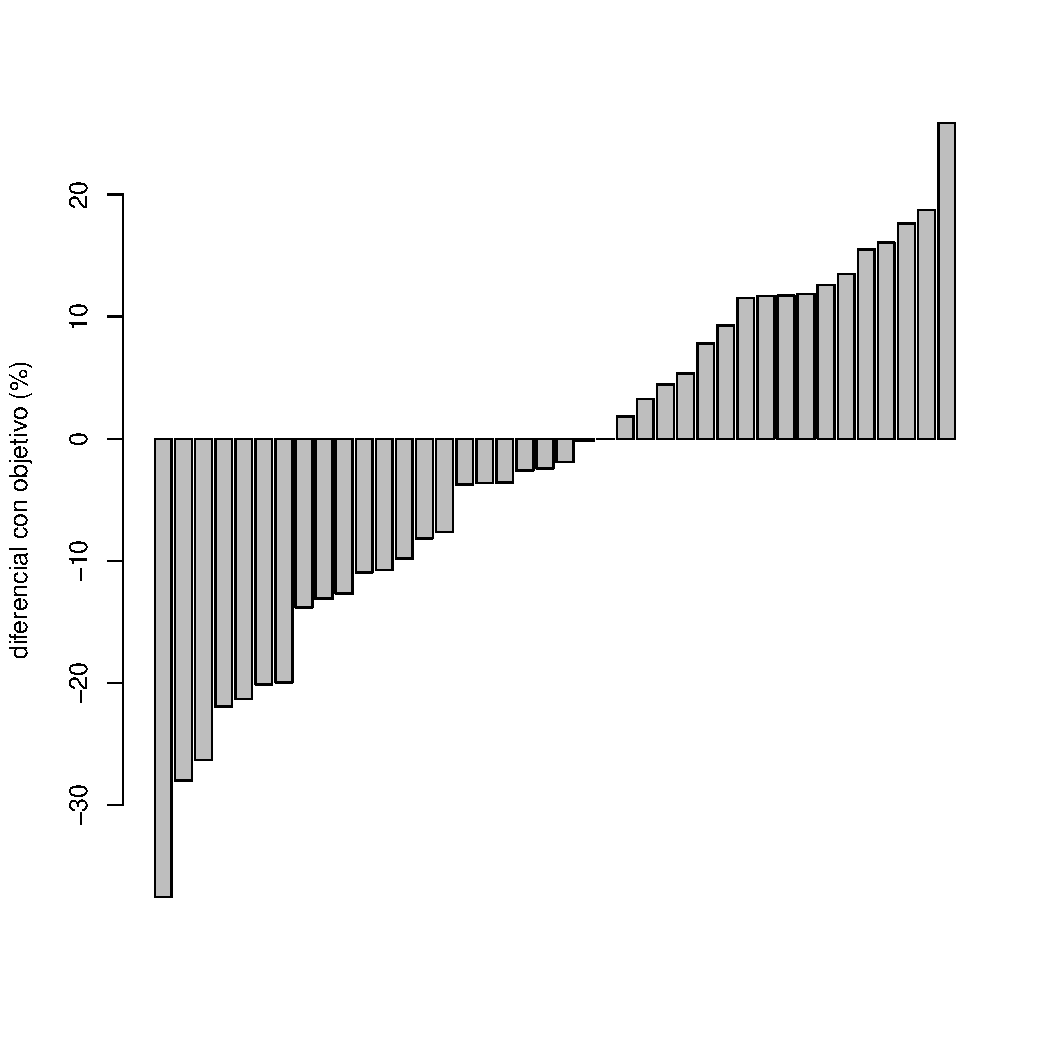
\includegraphics[width=.7\textwidth]{40dismex.pdf} \\
%  \includegraphics[width=.75\textwidth]{../../graphs/stateVetoHistogram.pdf} \\
 \end{center}


}
%%%%%%%%%%%%%%%%%%%%%%%%%%%%%%%%%%%%%%%%%%%%%%%%%%%%%%%%%%%%%%%%%%%%%%%%%%%%%%%%%%%%%%%%%%%%%%%% 
\frame {                      % SLIDE
    \frametitle{Del l\'apiz al internet}

\renewcommand{\theenumi}{\Alph{enumi}} %% use letters in this 1st-level enumerate

\be

\item Procesos manuales ($\leq 1978$)

  \bi

  \item Trazo a mano con informaci\'on demogr�fica

  \ei

\item Introducci�n de procesos de c\'omputo (1996, 2004)

  \bi

  \item Algoritmos de optimizaci\'on

  \item Criterios imparciales y sus limitaciones

  \ei

\item Internet, transparencia y participaci\'on ciudadana (?`$\geq 2013$?)

  \bi

  \item Difusi\'on de informaci�n \emph{ex-ante}

  \item Transparencia
  
  \item Potenciales afectados pueden sonar alarma a tiempo 

  \ei

\ee

}
%%%%%%%%%%%%%%%%%%%%%%%%%%%%%%%%%%%%%%%%%%%%%%%%
\frame {                      % SLIDE
     \frametitle{Resultados Dip.~Fed.~Edomex 2012}

\begin{center}

\begin{tabular}{lrrrr}

        & \%    & distritos  &        \% & en      \\
Partido & votos & que gan\'o & distritos & margen  \\ \hline
PAN     &    20 &    1       &         3 &   1     \\
PRI     &    43 &   26       &        65 &   5     \\
PRD     &    33 &   13       &        33 &  11     \\
\end{tabular}

\end{center}

}
% disn gano  2do  3ro mg12 mg23 dmgnal  |  disn gano  2do  3ro mg12 mg23 dmgnal
%    1  pri  pan  prd   35    5      0  |    21  pri  pan  prd   10    5      0
%    2  pri  prd  pan   12    7      0  |    22  pri  pan  prd    5    6      1
%    3  pri  pan  prd   32    9      0  |    23  pri  prd  pan   21    4      0
%    4  pri  prd  pan    6   12      1  |    24  pri  prd  pan   16   10      0
%    5  pri  prd  pan    9   19      0  |    25  pri  prd  pan   12   26      0
%    6  prd  pri  pan    0   14      1  |    26  pri  pan  prd   26    8      0
%    7  pri  prd  pan    3    6      1  |    27  pri  pan  prd   24    1      0
%    8  pri  prd  pan    6   21      1  |    28  pri  prd  pan   21    2      0
%    9  pri  prd  pan   33    5      0  |    29  prd  pri  pan    6   30      1
%   10  pri  prd  pan    7   21      0  |    30  prd  pri  pan   13   26      0
%   11  pri  prd  pan    7   19      0  |    31  prd  pri  pan   12   28      0
%   12  pri  prd  pan    2   21      1  |    32  prd  pri  pan    8   30      0
%   13  pri  prd  pan    4   26      1  |    33  pri  prd  pan    4   26      1
%   14  pri  prd  pan    6    3      1  |    34  pri  pan  prd   21    9      0
%   15  pan  pri  prd    3    6      1  |    35  pri  prd  pan   21   11      0
%   16  pri  prd  pan    6   23      1  |    36  pri  prd  pan   11   15      0
%   17  prd  pri  pan    1   27      1  |    37  pri  prd  pan    3   20      1
%   18  pri  pan  prd   15    0      0  |    38  prd  pri  pan   14   24      0
%   19  pri  prd  pan    4   12      1  |    39  pri  prd  pan    0   35      1
%   20  prd  pri  pan    5   26      1  |    40  pri  prd  pan   29    1      0
  

%%%%%%%%%%%%%%%%%%%%%%%%%%%%%%%%%%%%%%%%%%%%%%%%%%%%%%%%%%%%%%%%%%%%%%%%%%%%%%%%%%%%%%%%%%%%%%%%
\frame {                      % SLIDE
    \frametitle{Resultados seccionales}

 \begin{center}
  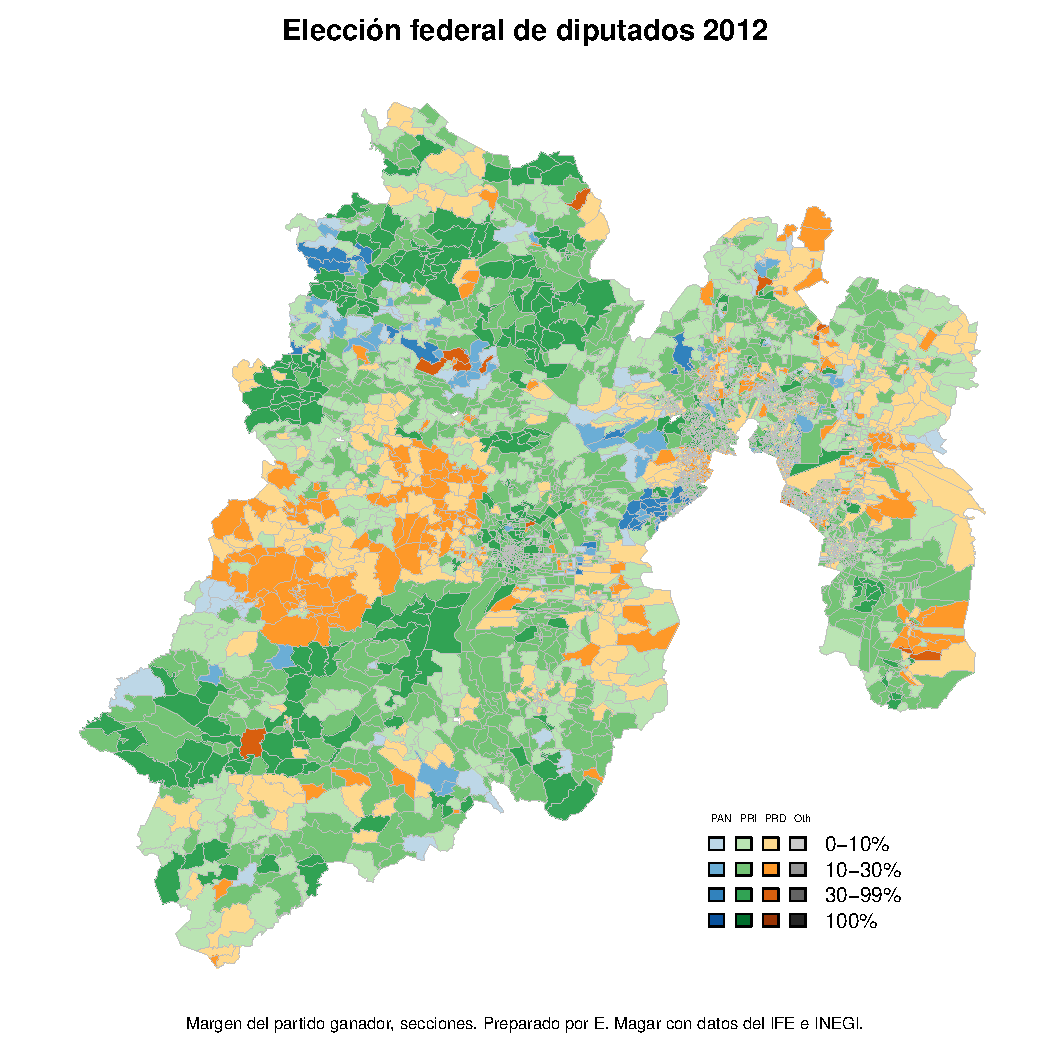
\includegraphics[width=.8\textwidth]{../shapes/mgSeccMapDipFed2012.pdf} \\
 \end{center}


}
%%%%%%%%%%%%%%%%%%%%%%%%%%%%%%%%%%%%%%%%%%%%%%%%%%%%%%%%%%%%%%%%%%%%%%%%%%%%%%%%%%%%%%%%%%%%%%%%
\frame {                      % SLIDE
    \frametitle{Resultados seccionales}

 \begin{center}
  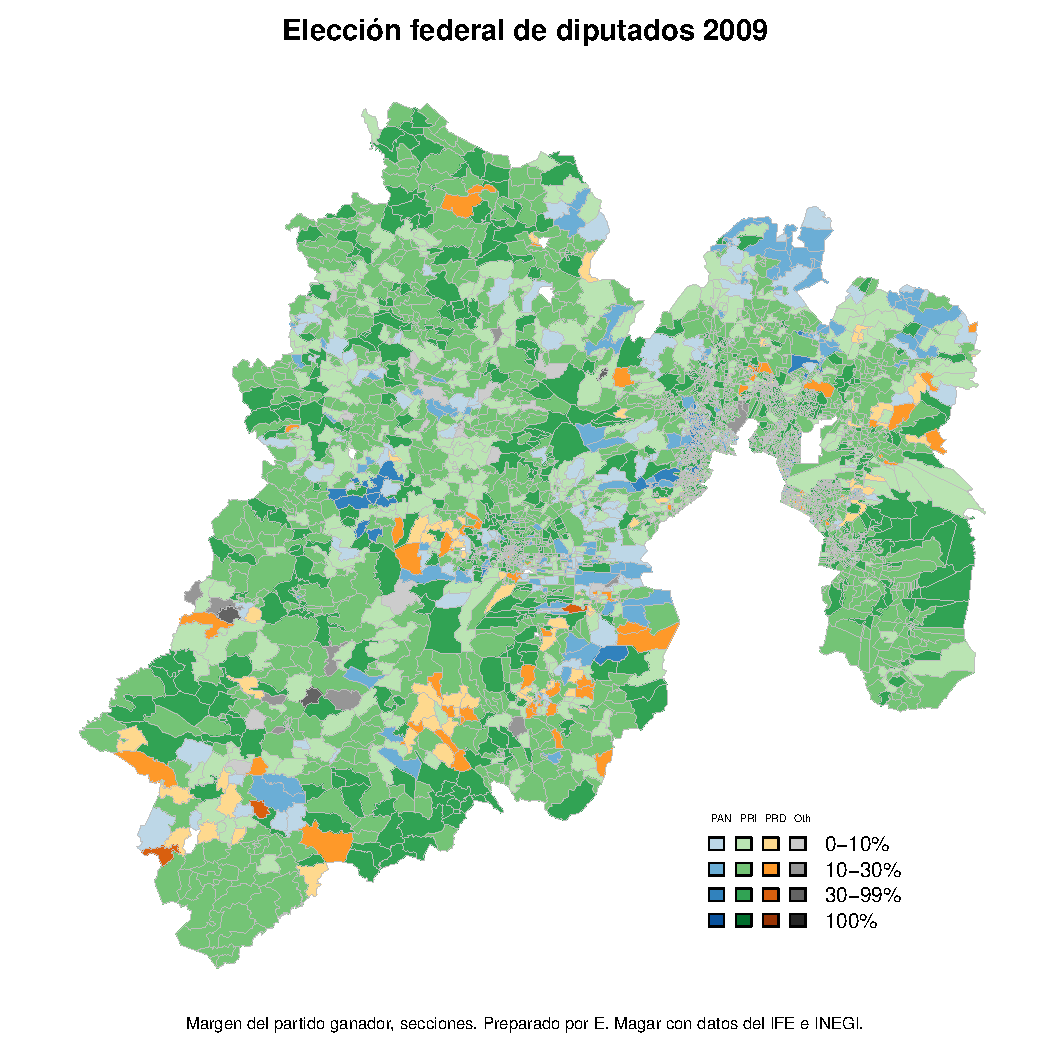
\includegraphics[width=.8\textwidth]{../shapes/mgSeccMapDipFed2009.pdf} \\
 \end{center}


}
%%%%%%%%%%%%%%%%%%%%%%%%%%%%%%%%%%%%%%%%%%%%%%%%%%%%%%%%%%%%%%%%%%%%%%%%%%%%%%%%%%%%%%%%%%%%%%%%
\frame {                      % SLIDE
    \frametitle{Resultados seccionales}

 \begin{center}
  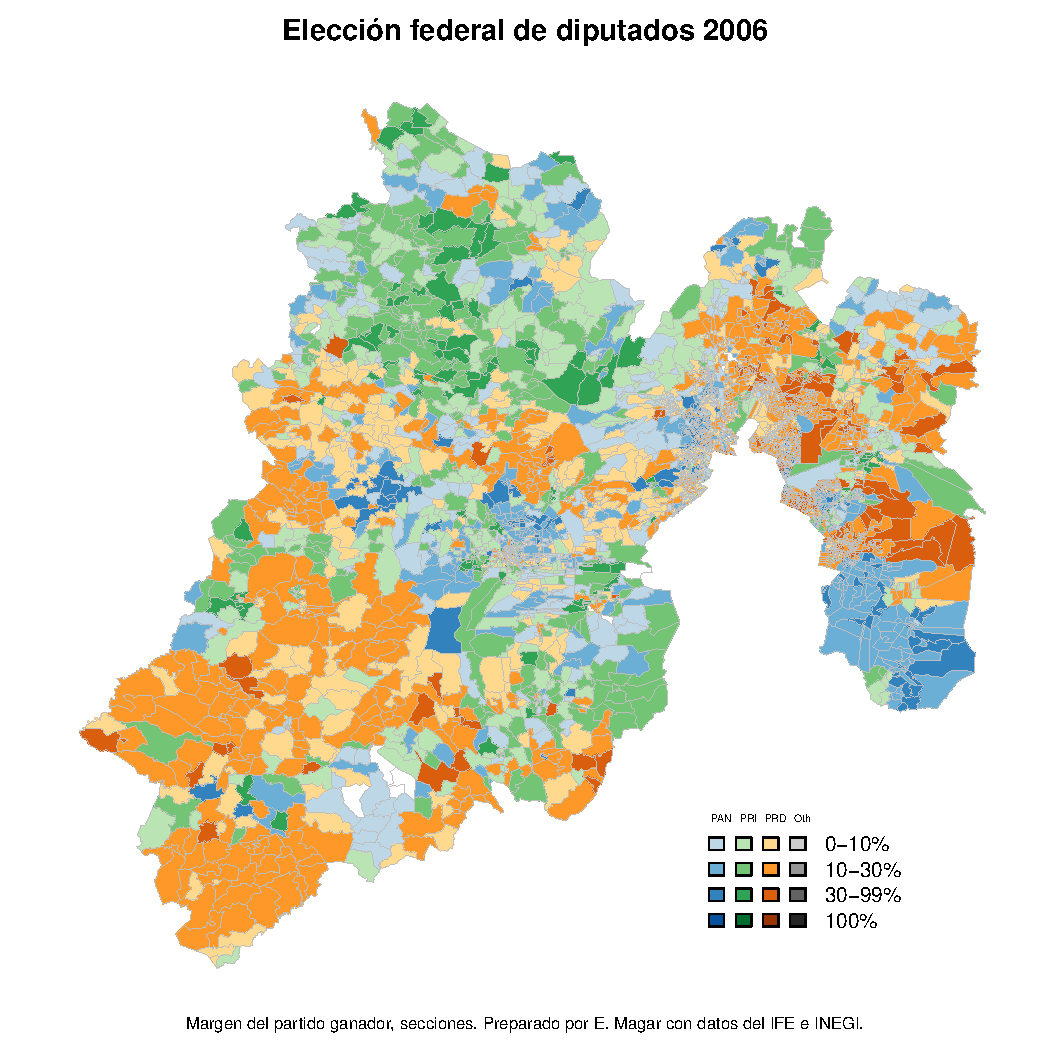
\includegraphics[width=.8\textwidth]{../shapes/mgSeccMapDipFed2006.pdf} \\
 \end{center}


}
%%%%%%%%%%%%%%%%%%%%%%%%%%%%%%%%%%%%%%%%%%%%%%%%%%%%%%%%%%%%%%%%%%%%%%%%%%%%%%%%%%%%%%%%%%%%%%%%
\frame {                      % SLIDE
    \frametitle{Agradecimientos}

Por apoyar con el pago de cuotas y transporte:

\bi

\item Consejo de Alumnos ITAM (Impulso)

\item Representaci�n de alumnos de Ciencia Pol\'itica ITAM (Caucus)

\item Jeff Weldon

\ei

\bigskip

Por atender nuestras molestas peticiones de �ltima hora:

\bi

\item Helena Varela

\item Alvaro L\'opez Lara

\ei

\bigskip

\begin{center}

\textbf{!`Muchas gracias!}

\end{center}
}


\end{document}
